\documentclass[11pt]{article}
\usepackage[left=2cm,right=2cm,top=2cm,bottom=2cm]{geometry}
\usepackage[utf8]{inputenc}
\usepackage{graphicx}
\usepackage{listings}
\usepackage[english]{babel}
\usepackage{comment}
\usepackage{hhline}
\usepackage{color}
\usepackage{url}
%\usepackage{csquotes}
\usepackage[backend=bibtex,style=verbose-trad2]{biblatex}
\bibliography{test} 
 
\newcommand{\HRule}{\rule{\linewidth}{0.6mm}}
 
\definecolor{codegreen}{rgb}{0,0.6,0}
\definecolor{codegray}{rgb}{0.5,0.5,0.5}
\definecolor{codepurple}{rgb}{0.58,0,0.82}
\definecolor{backcolour}{rgb}{0.95,0.95,0.92}
 
\lstdefinestyle{codestyle}{
    backgroundcolor=\color{backcolour},   
    commentstyle=\color{codegreen},
    keywordstyle=\color{magenta},
    numberstyle=\tiny\color{codegray},
    stringstyle=\color{codepurple},
    basicstyle=\footnotesize,
    breakatwhitespace=false,         
    breaklines=true,                 
    captionpos=b,                    
    keepspaces=true,                 
    numbers=left,                    
    numbersep=5pt,                  
    showspaces=false,                
    showstringspaces=false,
    showtabs=false,                  
    tabsize=2
}
 
\lstset{style=codestyle}

\begin{document}


\begin{titlepage}
\center % Center everything on the page
\HRule \\[0.4cm]
\textbf{\huge Assignment 8}\\[0.3cm] % course name
\textbf{\huge Python and Github}\\[0.3cm]
\HRule \\[1cm]


\textsc{\Large ELP-780}\\[0.4cm] % Course Code
\textsc{\huge Software Lab}\\[1cm] % course name
\textsc{\Large Ravi Singh Thakur}\\ [0.16cm]
\textsc{\Large 2017EET2840}\\[1cm]

\includegraphics[scale=1.25]{logo.jpg}\\[1cm]
\textbf{\Large Indian Institute Of Technology,}\\[0.2cm]
\textbf{\Large Delhi}\\[0.3cm]
{\Large \today}\\[3cm] % Date
\end{titlepage}
\pagebreak

\tableofcontents

\pagenumbering{arabic}
\newpage


\section{Problem Statement 1}
{

\subsection{Problem Statement}
\paragraph{ Find two largest crosses lengths of smart cell grid} 
\begin{itemize}
\item Input a 2D array of strings consisting of DULL and SMART cells and find crosses which will be of odd lengths.
\item Print largest two crosses found in matrix in non increasing order.
\end{itemize}
}

\subsection{Assumptions}
{
\begin{itemize}
\item Cells can either contains S or D character to represent SMART and DULL grid.
\item Dimensions of 2D matrix can not be greater than $105*105$.
\end{itemize}
}




\subsection{Algorithm Steps}
{
\begin{itemize}
\item If fourth column which is depicting plans in CDR is 1 then store it in plan1 file.
\item Repeat step 1 for plan2 and plan 3 as well.
\end{itemize}
\begin{itemize}
\item Search for MTC,MOC,SMSMT or SMSMO in fifth column and increment the value in corresponding variable.
\item Do above step for plan1,plan2 and plan3 file.
\end{itemize}
\begin{itemize}
\item Calculate MOC and SMS-MO charge according to plan rate table.
\item Print output in desired format.
\end{itemize}





\subsection{Input and Output Format}
{


\textbf{I/O format} 
\begin{itemize}
\item \subsubsection{Input Format}
\begin{itemize}
\item awk fileawk filenametxt 
\end{itemize}

\item \subsubsection{Output Format}
\begin{itemize}
\item All plan file in text format.
\item For each plan : Call type:Average Valeu
\item                 SMS type:Total value  
\item For part$1.3$
\item call type:charge
\item Sms type:charge
\item Total charge
\end{itemize}
\end{itemize}


}

\subsection{Difficulty faced}
{
\begin{itemize}
\item Process multiple files.
\end{itemize}
}



\subsection{Screenshots}
{
\begin{center}
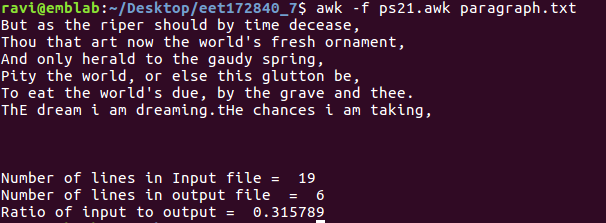
\includegraphics[scale=0.70]{sc1.png}


\end{center}
\newpage
}



\section{Problem Statement 2}
{

\subsection{Problem Statement}
\paragraph{ Search for a word in a file} 
\begin{itemize}
\item Search for the in file print that line.
\item Count number of occurance of the and print it.
\item count the number of lines in input and output files and find ratio.
\end{itemize}
} 

\subsection{Assumptions}
{
\begin{itemize}
\item the cannot be in the end of any line.
\item two words in file is separated by a space.
\end{itemize}
}




\subsection{Algorithm Steps}
{
\begin{itemize}
\item Search for the in file and print that line which contains it.
\item While reading each line containing the,keep on incrementing counter and at the end print it.
\item Find the number of lines in input and output file containing the and find its ratio.
\end{itemize}

\subsection{Input and Output Format}
{


\textbf{I/O format} 
\begin{itemize}
\item \subsubsection{Input Format}
\begin{itemize}
\item  awk fileawk filename 
\end{itemize}

\item \subsubsection{Output Format}
\begin{itemize}
\item First few lines are lines containing the from input file.
\item Counter value
\item Ratio
\end{itemize}
\end{itemize}


}

\subsection{Difficulty faced}
{
\begin{itemize}
\item Processing multiple files at a time.
\end{itemize}
}

\newpage
\subsection{Program Structure}
\begin{center}
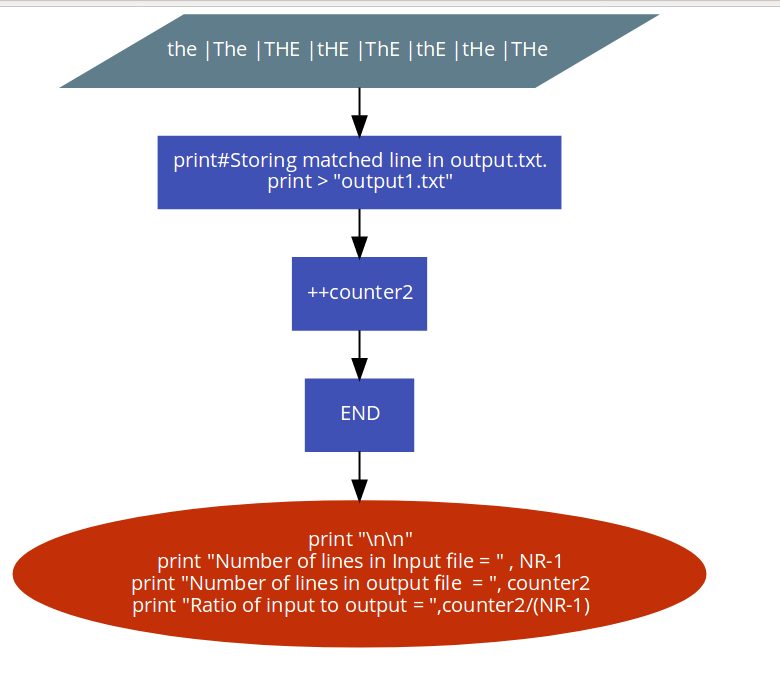
\includegraphics[scale=0.60]{fc2.png}
\end{center}
\newpage

\subsection{Screenshots}
{
\begin{center}
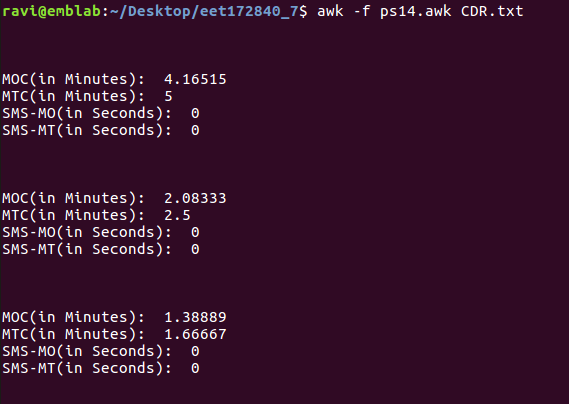
\includegraphics[scale=0.70]{sc21.png}
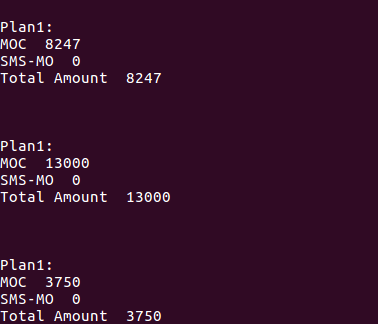
\includegraphics[scale=0.70]{sc22.png}

\end{center}
\newpage
}


\section{Appendix}
{
\textbf{Appendix-A : code for ps1.py}
\lstinputlisting[language=Python]{ps1.py}  

\newpage
\textbf{Appendix-B : code for ps2.py}
\lstinputlisting[language=Python]{ps2.py}

\newpage

}



\begin{thebibliography}{}
\bibitem{} 
https://stackoverflow.com/questions/44894083/awk-to-extract-lines-in-file-that-contain-matching-pattern-and-variable-digit
 
\bibitem{}
https://www.tutorialspoint.com/awk/awkbasicexamples.htm

\bibitem{} 
https://www.thegeekstuff.com/2010/02/awkconditionalstatements/
 


\end{thebibliography}
\end{document}